\section{Why the Band Selects Ill-Posed Problems}
\label{sec:mechanism}

\subsection{Solvable problems leave the band faster}
\label{sec:exit}

To isolate the filter from the proposer, we fix one pool of 1,158 first-round problems, label them all (639 solvable, 180 ambiguous, 339 unsolvable), and score it with the base model and the solvers of rounds one to five of one lineage$^{\dagger}$. The pool is that lineage's complete first-round output, so its round-1 solver trained on the pool's in-band problems; afterwards only the solver changes. The fraction of solvable problems in the band falls from 0.53 to 0.10, while that of unsolvable ones falls only from 0.72 to 0.60 (Figure~\ref{fig:mechanism}a). Solvable problems leave through the top: they start near the band's upper edge (mean agreement 0.71) and sharpen to 0.95, and unanimous problems are not admitted. Unsolvable problems gain agreement too (0.38 to 0.68), but start lower and mostly move up within the band. On a second, held-out pool the admitted ill-posed share rises from 56.2\% to 82.0\%, and post-trained models act as sharpened solvers (Appendix~\ref{app:results}).

An odds decomposition makes the link to the curriculum exact (Appendix~\ref{app:theory}). Let $\rho_S(t)$ and $\rho_I(t)$ be the fractions of solvable and ill-posed problems still in the band at round $t$, relative to round zero, and $s_t$ the ill-posed share of the admitted set. Then
\begin{equation}
\frac{\mathrm{odds}(s_t)}{\mathrm{odds}(s_0)} = \frac{\rho_I(t)}{\rho_S(t)} ,
\label{eq:odds}
\end{equation}
so the curriculum drifts toward ill-posed problems exactly when solvable ones leave the band faster; on the fixed pool, $\rho_S = 0.19$ and $\rho_I = 0.73$ at round five multiply the odds by 3.8. Why do solvable problems leave faster? If a problem's answer distribution sharpens as $q_t \propto q_0^{\beta^t}$ with $\beta > 1$, the probability that a problem whose modal answer has probability $q$ lands in the band, $m(q) \approx \Pr[2 \le \mathrm{Bin}(8, q) \le 6]$, satisfies $m'(q) = 56\, q (1-q) [ (1-q)^5 - q^5 ] < 0$ for $q > \frac{1}{2}$, so once its modal share passes one half, sharpening pushes a problem out of the band, faster for a larger rate $\beta$ (likewise for the R-Zero code's filter; Appendix~\ref{app:theory}).

\begin{figure}[t]
\centering
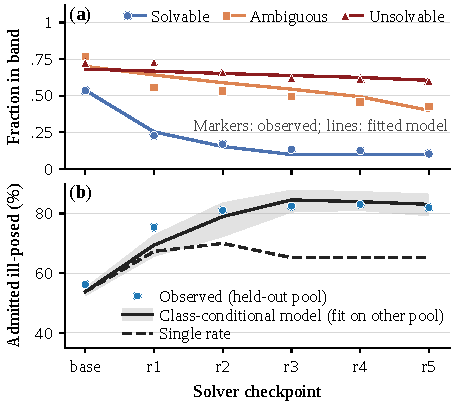
\includegraphics[width=0.85\columnwidth]{figures/fig2_mechanism.pdf}
\caption{The filter, isolated. (a)~Fraction of each class of the fixed pool inside the band (markers: observed; lines: fitted class-conditional sharpening model). (b)~Ill-posed share admitted from the held-out pool: observed, predicted by the model fitted on the fixed pool (shaded: 95\% bootstrap interval) and by a single rate.}
\label{fig:mechanism}
\end{figure}

\subsection{Each class sharpens at its own rate}
\label{sec:law}

We describe the exit with a class-conditional sharpening model, with one rate $\beta_c$ per class, fitted to the fixed pool$^{\dagger}$, reconstructing each problem's base answer distribution from its base agreement (Appendix~\ref{app:theory}; refitted after a numerical fix). Solvable problems sharpen fastest ($\beta_S = 3.75$, 95\% CI $[2.65, 4.40]$), ambiguous ones more slowly ($\beta_A = 1.60$ $[1.50, 1.75]$) and unsolvable ones slowest ($\beta_U = 1.40$ $[1.05, 1.55]$); $\beta_S$ exceeds both other rates in every bootstrap resample, also with the exact modal count of eight samples in place of the mode's binomial count, although the values then change ($\beta_S = 7.5$; Appendix~\ref{app:theory}): the rates are an ordering, not calibrated parameters. Applied without refitting to the second pool (another lineage), the model tracks the admitted ill-posed share with a mean absolute error of 2.4 points over six checkpoints (2.5 with the modal count)$^{\dagger}$; its largest error underestimates the first-round jump (Figure~\ref{fig:mechanism}b), and its late plateau rests on problems with a tied base mode, which it never sharpens. A single rate fits each class far worse and plateaus near 65\% instead of 82\%. In two further models the pre-specified class ordering holds: $\beta_S = 2.55 > \beta_A = 1.50 > \beta_U = 1.45$ for Qwen3-8B, and $2.5 > 1.1 > 1.0$ for Phi-4-mini. Without the model, too, solvable problems stay in the band less often than unsolvable ones of equal base agreement, in every round and model$^{\dagger}$.

\subsection{The band keeps unresolved problems}
\label{sec:hard}

UMWP lets us ask with human labels whether the band prefers ill-posed problems or merely hard ones. Under the filter reading, unanswerable questions stay in the band 1.32 times as often as answerable ones after three rounds at matched base agreement (95\% CI $[1.27, 1.38]$), but not markedly more often than \emph{hard} answerable questions, which the base model solves in at most three of eight samples: the matched ratio reaches 1.25 in only two of ten lineages. What separates the two is how they leave$^{\dagger}$: for Qwen3-4B, 195 of the 209 exits of hard answerable questions are solves by round three (fresh base-model samples show none), while unanswerable ones leave less often, almost always as a self-consistent answer (483 of 512 exits). Under the strict reading, which the filter does not apply, 344 of their 658 exits are declines. The band keeps whatever training has not resolved; among model-written problems, that is mostly the ill-posed ones.

\subsection{Ill-posed problems disagree over readings}
\label{sec:readings}

Hard and ill-posed problems also disagree for different reasons. We sampled eight solutions to each of 112 unanswerable UMWP questions and 112 hard answerable ones matched on base agreement; LLM labellers, blind to model, round and answerability, marked the distinct readings or completions of the text that the solutions adopt and the source of disagreement (Appendix~\ref{app:readings}). At base, unanswerable questions disagree over readings in 94\% of cases, against 26\% for hard answerable questions, which disagree through computation errors (difference $+0.68$, 95\% CI $[0.59, 0.77]$); two human annotators confirm this on 184 of the questions (88\% against 16\%; Appendix~\ref{app:readings}). This fits the rates of \S\ref{sec:law}, although such observational labels cannot establish their cause: majority voting reinforces the most frequent answer, which for a solvable problem is the correct one, shared across reasoning paths while errors scatter, whereas each reading of an ill-posed problem yields its own self-consistent answer, so reinforcement is split among competing modes. Training still narrows the readings: after five rounds, the readings per unanswerable question fall from 3.9 to 2.7--3.2, and all eight answers coincide for 1.8--4.5\% of the questions, against none at base; hard answerable questions stay at about 1.35.
